\graphicspath{{chapters/07/images/}}
\chapter{Fetal healing}

\section{Introduction}
Regeneration of amputated limb can occur at an adult stage in amphibians and fish.
This complex process is enabled by specific tissue regeneration mechanisms.
For instance,  in adults of Homo Sapiens the liver regenerates spontaneously.
However, we have little capacity to regenerate tendons and ligaments.

	\subsection{Scarring}
	A scar is a densely packed disorganized collagen bundle, with absence of hair follicles, sebaceous glands and other appendages.
	Scarring and fibrosis dominate some diseases in every branch of medicine and surgery: for example skin incisions heal with scars and cause pathological processes like keloids or hypertrophic scars.

	\subsection{Adult scarring}
	The mechanism of scar formation involves:

	\begin{multicols}{2}
		\begin{enumerate}
			\item Inflammation.
			\item Fibroplasia.
			\item Formation of granulation tissue
			\item scar maturation.
		\end{enumerate}
	\end{multicols}

	The acute inflammatory response due to pro-inflammatory mediators is followed by the proliferation of fibroblasts, the cells responsible for synthesizing various tissue components, including collagen and fibrin.
	During the acute inflammatory phase, circulating progenitor cells migrate to injured tissue.
	Rapid cellular proliferation occurs, which ultimately results in the formation of new blood vessels and epithelium.
	Fibroblasts then differentiate into myofibroblasts, which are the cells responsible for collagen deposition and wound contraction.
	Scar formation ultimately results from excess accumulation of an unorganized extracellular matrix.
	Although scar remodelling occurs for months to years after the initial injury, complete restoration of the normal extracellular matrix architecture is never achieved.

\section{Embryonic healing}
In contrast to adult wounds, early gestation fetal skin wounds repair rapidly and in the absence of scar formation.
The fetus is able to regenerate tissues by assembling collagen fiber in a well organised structure.
Cellular and matrix event in fetal repair may provide insights to help to modulate adult wound repair to become more fetal-like.

	\subsection{Fetal extracellular matrix}
	To achieve scarless healing the embryonic development procedure should be mimicked.
	In this procedure the ECM is elaborated in parallel with cell differentiation and growth.
	In particular, the aim is not to obtain a normal ECM analogue of the mature scaffold, but a wound bed matrix analogue suitable for regeneration.
	Collagen represents a mature scaffold, forming a microenvironment suitable for fully differentiated cells.
	If the scaffold is built based on collagen type I, cells which don't usually reside in an ECM made extensively of collagen type I will not interact with the surface, leading to a pathological response.
	For example chondrocytes usually interact with collagen type II, so if collagen type I is present cells will form fibrocartilage.

		\subsubsection{Fetal ECM components}
		The fetal extracellular matrix is optimized to facilitate cellular migration and proliferation, which may have important implications in wound healing.

		\begin{multicols}{2}
			\begin{itemize}
				\item High content of collagen type II and V, increased collagen synthesis.
				\item In scarless fetal wounds, the hyaluronic acid content of the extracellular matrix is increased more rapidly than in adult wounds becoming a major component of the ECM.
				\item Scarless fetal wounds have an enhanced ability to up-regulate extracellular matrix adhesion proteins, such as tenascin and fibronectin.
				\item Fibromodulin inactivates transforming growth factor TGF-$\beta$, a key cytokine involved in wound healing, and has been shown to have an antiscarring effect during wound repair.
				\item Non-sulfonated GAGs.
			\end{itemize}
		\end{multicols}

	\subsection{Fetal mediators of scarless repair}
	Fetal mediators of scarless repair are:

	\begin{multicols}{2}
		\begin{itemize}
			\item Lack of inflammation: decreased platelet degranulation and aggregation and presence of anti-inflammatory cytokines.
			\item Fibrobrlast cells with high migration rate affecting collagen depth and cross linking.
			\item Increased number of HA receptors.
			\item Myofriboblasts appear earlier and then disappear.
		\end{itemize}
	\end{multicols}

	\begin{figure}[h]
		\centering
		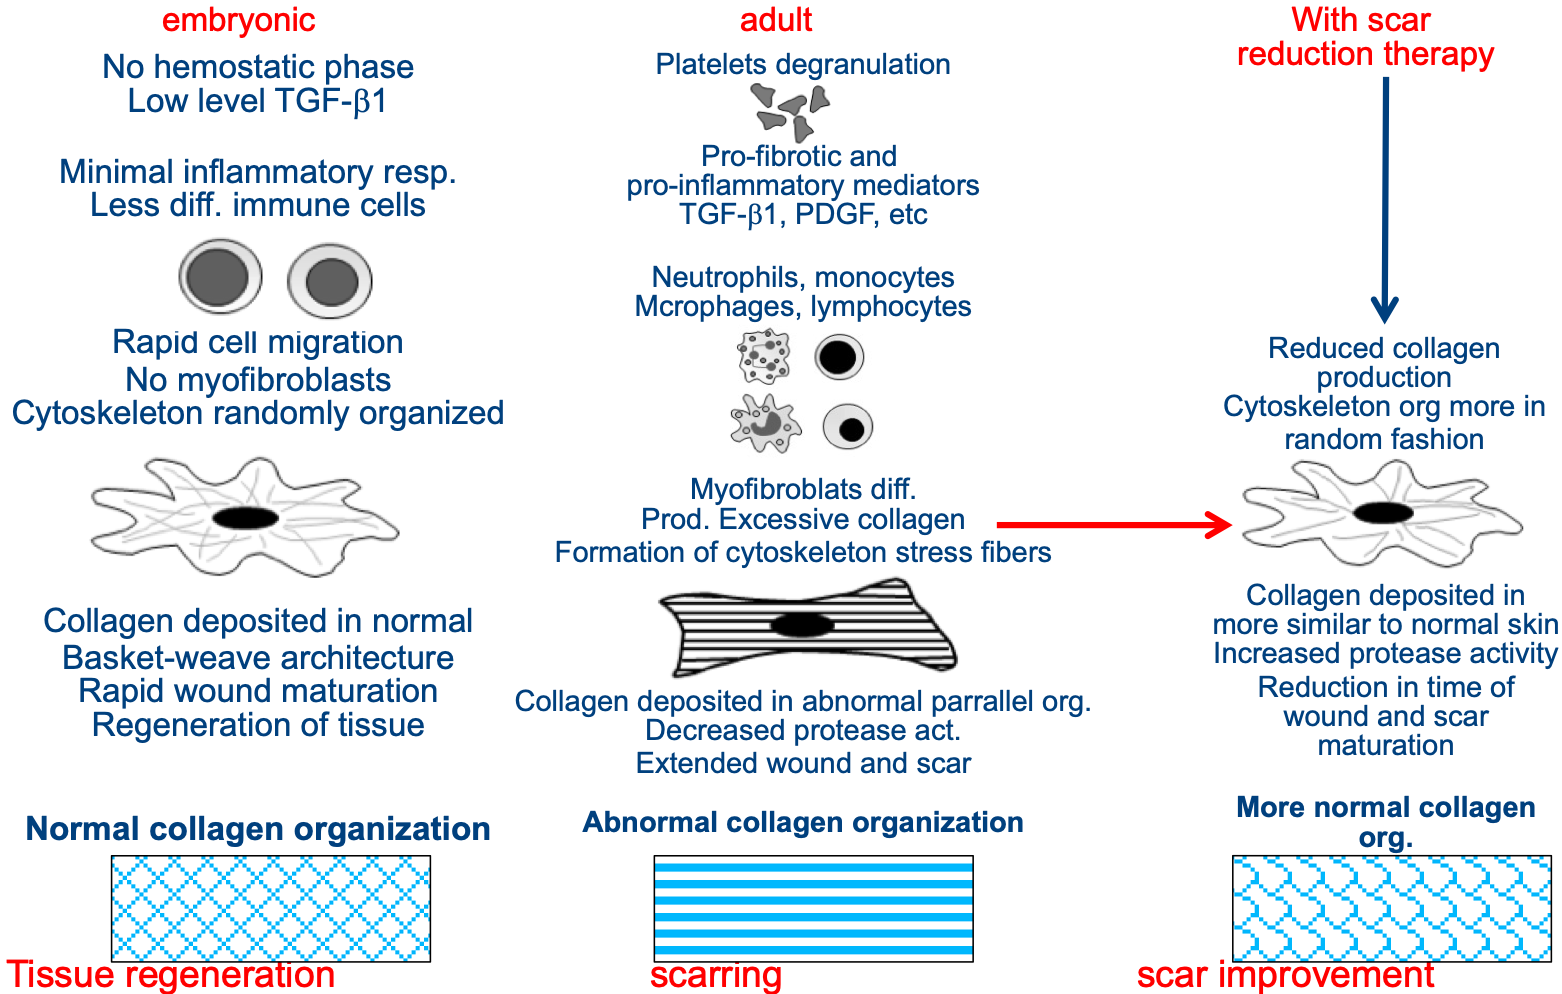
\includegraphics[width=0.5\textwidth]{scar.png}
		\caption{\label{fig:scar}A lesson from fetal healing: scarless regeneration}
	\end{figure}

	\subsection{Hyaluronan}
	Hyaluronan is a hydrated gelatinous material synthesized from the basal side of an epithelial sheet.
	It creates a cell-free space into which cells can proliferate and migrate, perform the diffusion of nutrients and metabolites.
	It is able to resist compressive forces and acts as space filling material in embryogenesis.
	It is degraded by hyaluronidase.

		\subsubsection{Composition}
		Hyaluronian is composed by the simplest GAG with a very long chain length of 25000 disaccharide units.
		It lacks sulfated sugars and is usually not attached to protein which are used as filler.
		The high negative charges on the glucuronic acid attract Na+ ions and water.

	\subsection{Collagen assembly}
	Collagen type III is involved in structural maintenance in expansible organs like smooth muscle, blood vessels and connective tissue and is prevalent in fetal healing.
	Collagen type V instead is responsible for fibril formation in skin, bones and fibrocartilage.
	In particular, collagen fibrils have a high content of collagen type III and IV.
	Collagen type III is important in generating a more reticular pattern of fibre deposition.
	Moreover a majority of non-crosslinked collagen in early fetal wounds produces a more flexible matrix, contributing to scarless repair.
